\section{Algoritmia}
\subsection{Conceptos}
\subsubsection{Algoritmo}
Secuencia de pasos a seguir para resolver un problema. Un algoritmo tiene las siguientes características:
\begin{itemize}
\item Finitud
\item Exactitud
\item Sin Ambiguedades
\end{itemize}
Esquema de un algoritmo:
\begin{itemize}
\item \textbf{Entrada:} Conjunto de Datos a ser procesado. Donde la cantidad de datos es representada por: $n$.
\item \textbf{Salida:} Conjunto de datos resultantes del proceso.
\item \textbf{Proceso:} Conjunto de Instrucciones para transformar la entrada en la salida.
\end{itemize}
\subsection{Tiempo de Ejecución}
Denotado por:
$$T_A(n)$$
Es el tiempo que le toma a un algoritmo $A$ procesar una entrada de tamaño $n$. Para determinar esto es necesario diferenciar: \textit{Cantidad de Operaciones} y \textit{Cantidad de Instrucciones.}
\subsubsection{Cantidad de Operaciones}
Para entender este punto basta ver el siguiente ejemplo:
\lstinputlisting[language=C++]{Codigos/codigo_intro.cpp}
Donde la cantidad de operaciones es de tres, estas son el producto de de \texttt{b*c}, esto con la suma de \texttt{a} forman dos operaciones la tercera operación es todo eso asignado a \texttt{x}.
\subsubsection{Cantidad de Instrucciones}
Para el mísmo ejemplo anterior:
\lstinputlisting[language=C++]{Codigos/codigo_intro.cpp}
En este caso la cantidad de \textit{Instrucciones} es de una.
\subsection{Cálculo de $T(n)$}
Para el cálculo de tiempo tendremos dos clasificaciones:
\begin{enumerate}
\item \textbf{Algoritmos Iterativos:} Usando tablas de conteo.
\item \textbf{Algoritmos Recursivos:} Mediante Ecuaciones de Recurrencia.
\end{enumerate}
\subsection{Clasificación de Algoritmos por su Grado de Complejidad}
\begin{multicols}{2}
\begin{itemize}
\item Algoritmos Constantes
\item Algoritmos Lineales
\item Algoritmos Logarítmicos
\item Algoritmos Cuadráticos
\end{itemize}
\columnbreak
\begin{itemize}
\item Algoritmos $n$-logarítmicos
\item Algoritmos Cúbicos
\item Algoritmos Exponenciales
\item Algoritmos Factoriales
\end{itemize}
\end{multicols}


\begin{figure}[h]
\centering
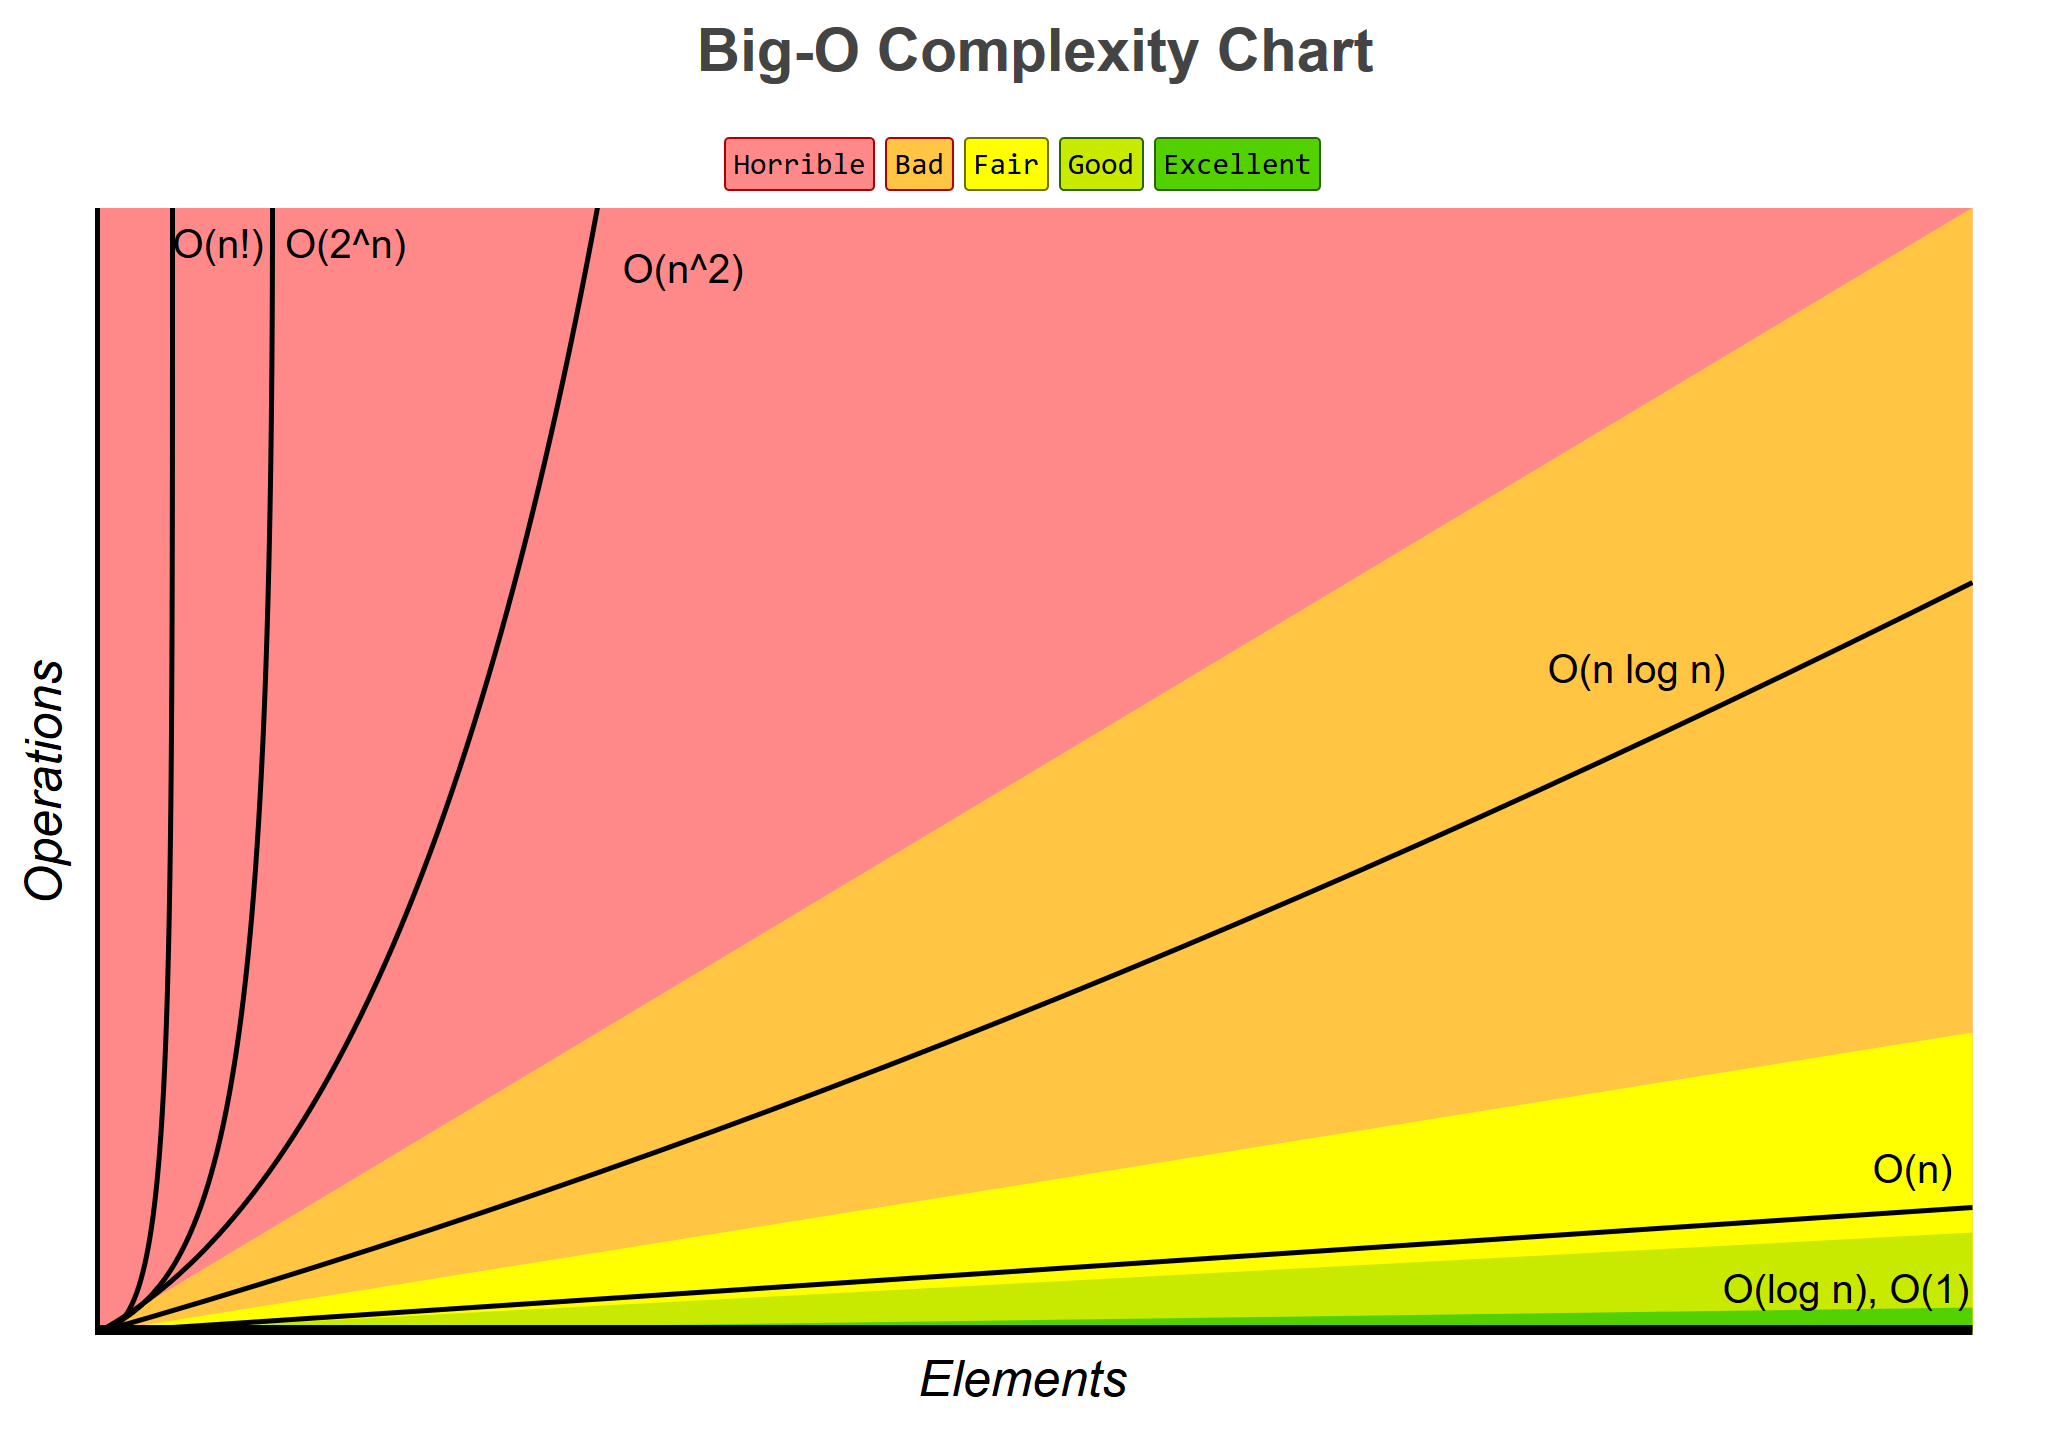
\includegraphics[scale=0.20]{BigO}
\captionsetup{justification=centering}
\caption[caption]{\footnotesize Gráfica que expresa el crecimiento de las operaciones para cada Grado de Complejidad. \\ \textbf{Fuente:} \texttt{http://bigocheatsheet.com}}
\end{figure}
\section{Cálculo de Tiempo}
\subsection{Algoritmos Constantes}
Tiene la siguiente forma:
$$T(n)=C \hspace{1cm} \textrm{donde $C$ es una Constante}$$
Son algoritmos que no contienen ciclos (que se ejecuten) y tarda siempre el mismo tiempo.
\subsubsection{Ejemplos}
\begin{enumerate}
\item Función que Intercambia dos variables por referencia:
\lstinputlisting[language=C++]{Codigos/intercambiar.cpp}
Podemos ver que las únicas líneas que contienen instrucciones son las líneas \texttt{3,4} y \texttt{5}. Y estas siempre serán las instrucciones que se ejecutaran, sin importar los datos de la función. Por lo tanto:
$$T_{intercambiar}(2)=3$$
\item Función que devuelve el mayor de los datos de un vector ordenado:
\lstinputlisting[language=C++]{Codigos/mayor.cpp}
En esta función no hay mucho misterio, si vemos la línea \texttt{3} sabemos que:
$$T_{mayor}(n)=1$$
\end{enumerate}
\subsection{Algoritmos Lineales}
Tienen la siguiente forma:
$$T(n)=An+B$$
\subsubsection{Ejemplos}
\begin{enumerate}
\item Función que devuelva la suma de los elementos de un arreglo:
\lstinputlisting[language=C++]{Codigos/suma_elementos.cpp}
Realizamos una tabla de conteo para cada línea que contenga instrucciones:
\begin{center}
\begin{tabular}{|c|c|}
\hline 
$l$ & $T(l)$ \\ 
\hline 
\texttt{4} & $2$ \\ 
\texttt{5} & $n+1$ \\ 
\texttt{7} & $n$ \\ 
\texttt{8} & $n$\\ 
\texttt{10} & $1$\\ 
\hline 
\end{tabular} 
\end{center}
Finalmente el tiempo de este ejemplo es la suma de los tiempos de todas las líneas, esto es: 
$$T_{SumaElementos}(n)=3n+4$$ 
Esto quiere decir que por ejemplo, si tuvieramos un vector con cuatro elementos, el tiempo de este algoritmo sería:
$$T_{SumaElementos}(4)=3\cdot 4+4=16$$
Esto significa que le tomara 16 instrucciones sumar un vector de cuatro elementos.
\end{enumerate}
